% ==============================================
% CFD Tutorial Template: OpenFOAM Terminal Basics
% Class: scrartcl (KOMA-Script) - optimized for tutorials
% Content: pitzDaily with simpleFoam
% ==============================================

\documentclass[
parskip=half,      % Space between paragraphs (better for steps)
DIV=12,            % Optimal margins for readability
headings=normal,   % Professional heading sizes
fontsize=11pt,     % Slightly larger for screen reading
english            % Language setting
]{scrartcl}

\input{../preamble.tex}
\usetikzlibrary{intersections}

% ========== DOCUMENT START ==========
\begin{document}
	
	% ========== TITLE PAGE ==========
	\title{Tutorial \#4: 3D Y-Pipe}
	\subtitle{Incompressible Steady Flow: 3D Y-Pipe with simpleFOAM in terminal}
	\subject{Open Source CFD }
	\author{Robert Castilla \\ Department of Fluid Mechanics}
	\date{2025-26 \\ Version 1.0}
	\publishers{Learning Objectives:
		\begin{itemize}
			\item Create a complex 3D geometry with sketch and additive pipe with FreeCAD
			\item Generate high quality triangulated surface
			\item Mesh a 3D geometry with \texttt{snappyHexMesh}
			\item Setup a case with multiple inlets
			\item Analyze flow and pressure drop
			\item Visualize 3D results with \texttt{paraview}
	\end{itemize}}
	
	\maketitle
	
	% ========== ABSTRACT ==========
	\begin{abstract}
		This tutorial introduces the fundamental workflow of Computational Fluid Dynamics (CFD) for a 3D geometry. We simulate the flow in a Y-shaped pipe junction. You will create the 3D geometry with FreeCAD, generate a high-quality triangulated surface file. Then, with OpenFOAM and CLI (Command Line Interface in terminal), mesh the geometry, run the steady simulation. Finally, post-process of the results will be made with CLI and \texttt{paraview}. 
	\end{abstract}
	
	\tableofcontents
	\newpage
	
	\section{Introduction}
	
	The Y-pipe consists of:
	\begin{itemize}
		\item Main pipe: 250 mm long, 100 mm diameter
		\item Secondary branch: 500 mm long branch at 90°, 100 mm diameter
		\item Inlet branch: 250 mm long, 50 mm diameter
	\end{itemize}
	
	An scheme of the Y-pipe is shown in Figure \ref{fig:ypipe}
	\begin{figure}[h]
		\centering
		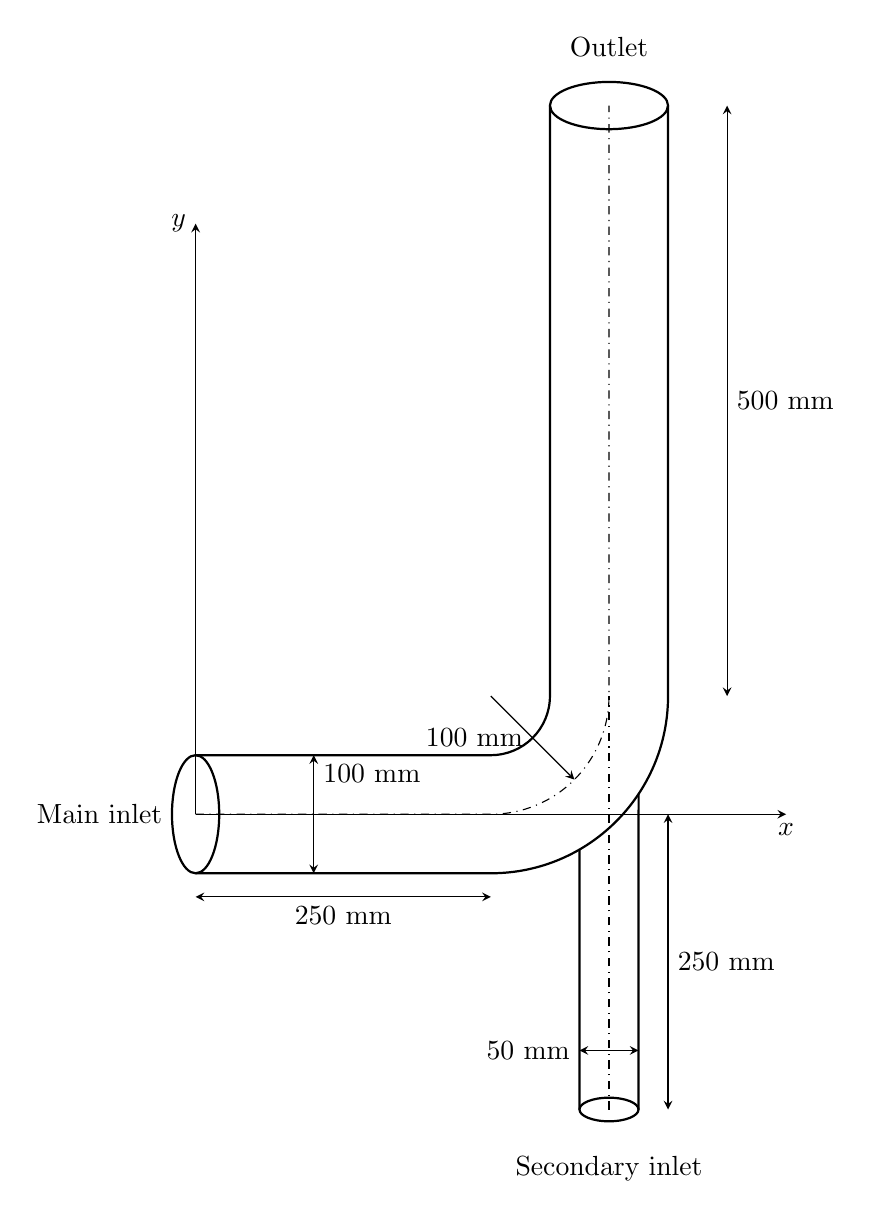
\begin{tikzpicture}[>=stealth,scale=1.5]
			\draw[->] (0,0) --++(5,0) node[below]{$x$};
			\draw[->] (0,0) --++(0,5) node[left]{$y$};
			\draw[dashdotted] (0,0) --++(2.5,0) arc [start angle=-90,end angle=0,x radius=1,y radius=1]
			--++(0,5);
			\draw[dashdotted] (3.5,-2.5) --++(0,3.5);
			% Main pipe (horizontal)
			\draw[thick] (0,0) ellipse (0.2 and 0.5);
			\draw[thick, name path = arc] (0,-.5) --++ (2.5,0) arc [start angle=-90,end angle=0,x radius=1.5,y radius=1.5] 
			--++(0,5);
			\draw[thick] (0,0.5) --++(2.5,0) arc [start angle=-90,end angle=0,x radius=0.5,y radius=0.5]
			--++(0,5);
			\draw[thick] (3.5,6) ellipse (0.5 and 0.2);
			
			% Secondary inlet 
			\path[name path = line1] (3.25,-2.5) --++(0,5);
			\path[name path = line2] (3.75,-2.5) --++(0,5);
			\path [name intersections={of=arc and line1, by=intersect1}];
			\path [name intersections={of=arc and line2, by=intersect2}];
			\draw[thick] (3.5,-2.5) ellipse (0.25 and 0.1);
			\draw[thick] (3.25,-2.5) -- (intersect1)  ;
			\draw[thick] (3.75,-2.5) -- (intersect2)  ;
			% Labels
			\node at (-0.2,0)[left] {Main inlet};
			\node at (3.5,-3) {Secondary inlet};
			\node at (3.5,6.5) {Outlet};
			% dimensions
			\draw[<->](0,-0.7)--++(2.5,0) node[midway, below]{250 mm};
			\draw[<->](4.5,1)--++(0,5) node[midway, right]{500 mm};
			\draw[<->](4,-2.5)--++(0,2.5) node[midway, right]{250 mm};
			\draw[<->](1,-0.5) --++ (0,1) node[below right] {100 mm};
			\draw[<->](3.75,-2) --++ (-0.5,0) node[left] {50 mm};
			\draw[->](2.5,1) --++ (-45:1) node[midway, left] {100 mm};
			
		\end{tikzpicture}
		\caption{Y-pipe geometry schematic}
		\label{fig:ypipe}
	\end{figure}
	
	\section{Generation of the geometry}
	
	\subsection{The solid}
	
	First, open a new \texttt{Part design} and an sketch in the XY plane. Draw the center
	line of the main pipe and the branch. It is composed of an horizontal line of 
	\qty{250}{mm} long, an arc of radius \qty{100}{mm} and a vertical line \qty{500}{mm}
	long. Don't worry about the dimensions and tangent lines when drawing the sketch, they 
	can define later. When the sketch is completely defined, it becomes green, 
	and it can be closed.
	
	\begin{figure}[h]
		\centering
		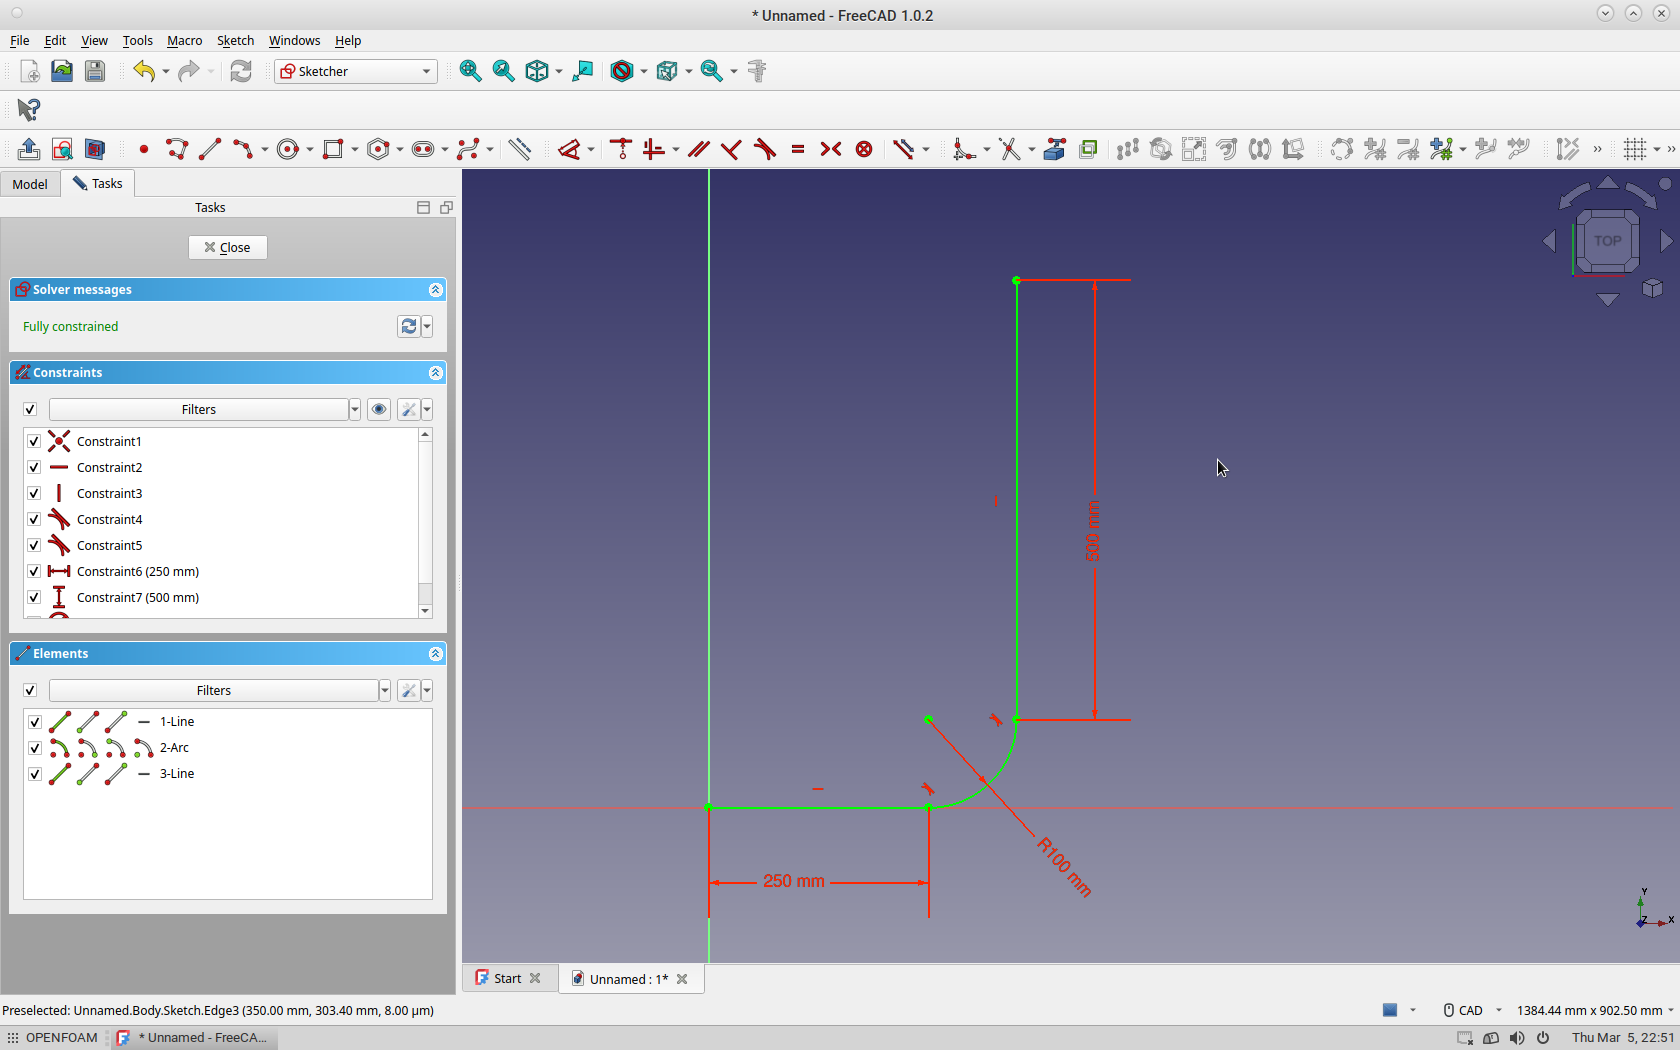
\includegraphics[width=0.7\linewidth]{sketch}
		\caption{First sketch.}
		\label{fig:sketch}
	\end{figure}
	
	Draw another sketch, with just a circle of radius \qty{50}{mm}, in the YZ plane
	
	\begin{figure}[h]
		\centering
		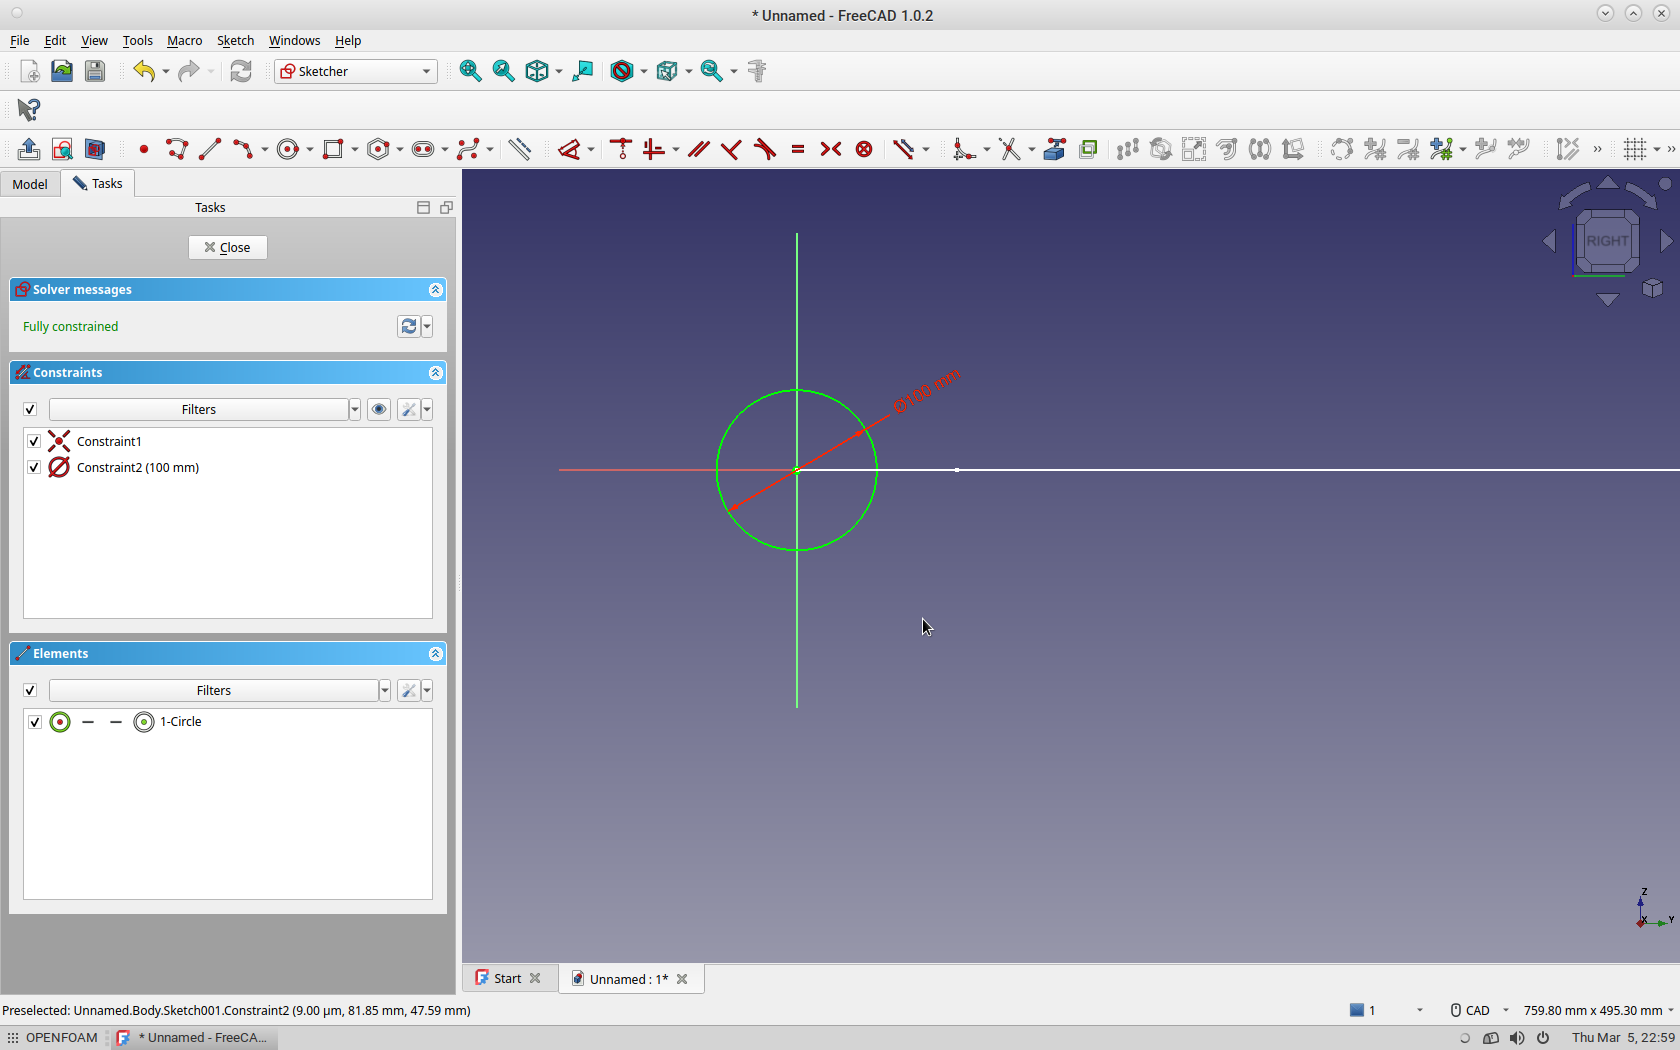
\includegraphics[width=0.7\linewidth]{sketch1}
		\caption{Sketch for 100 mm circle in YZ plane}
		\label{fig:sketch1}
	\end{figure}
	
	Select both sketches and make an \texttt{Additive pipe}. The result should be like in 
	Figure \ref{fig:pipe1}.
	
	\begin{figure}[h]
		\centering
		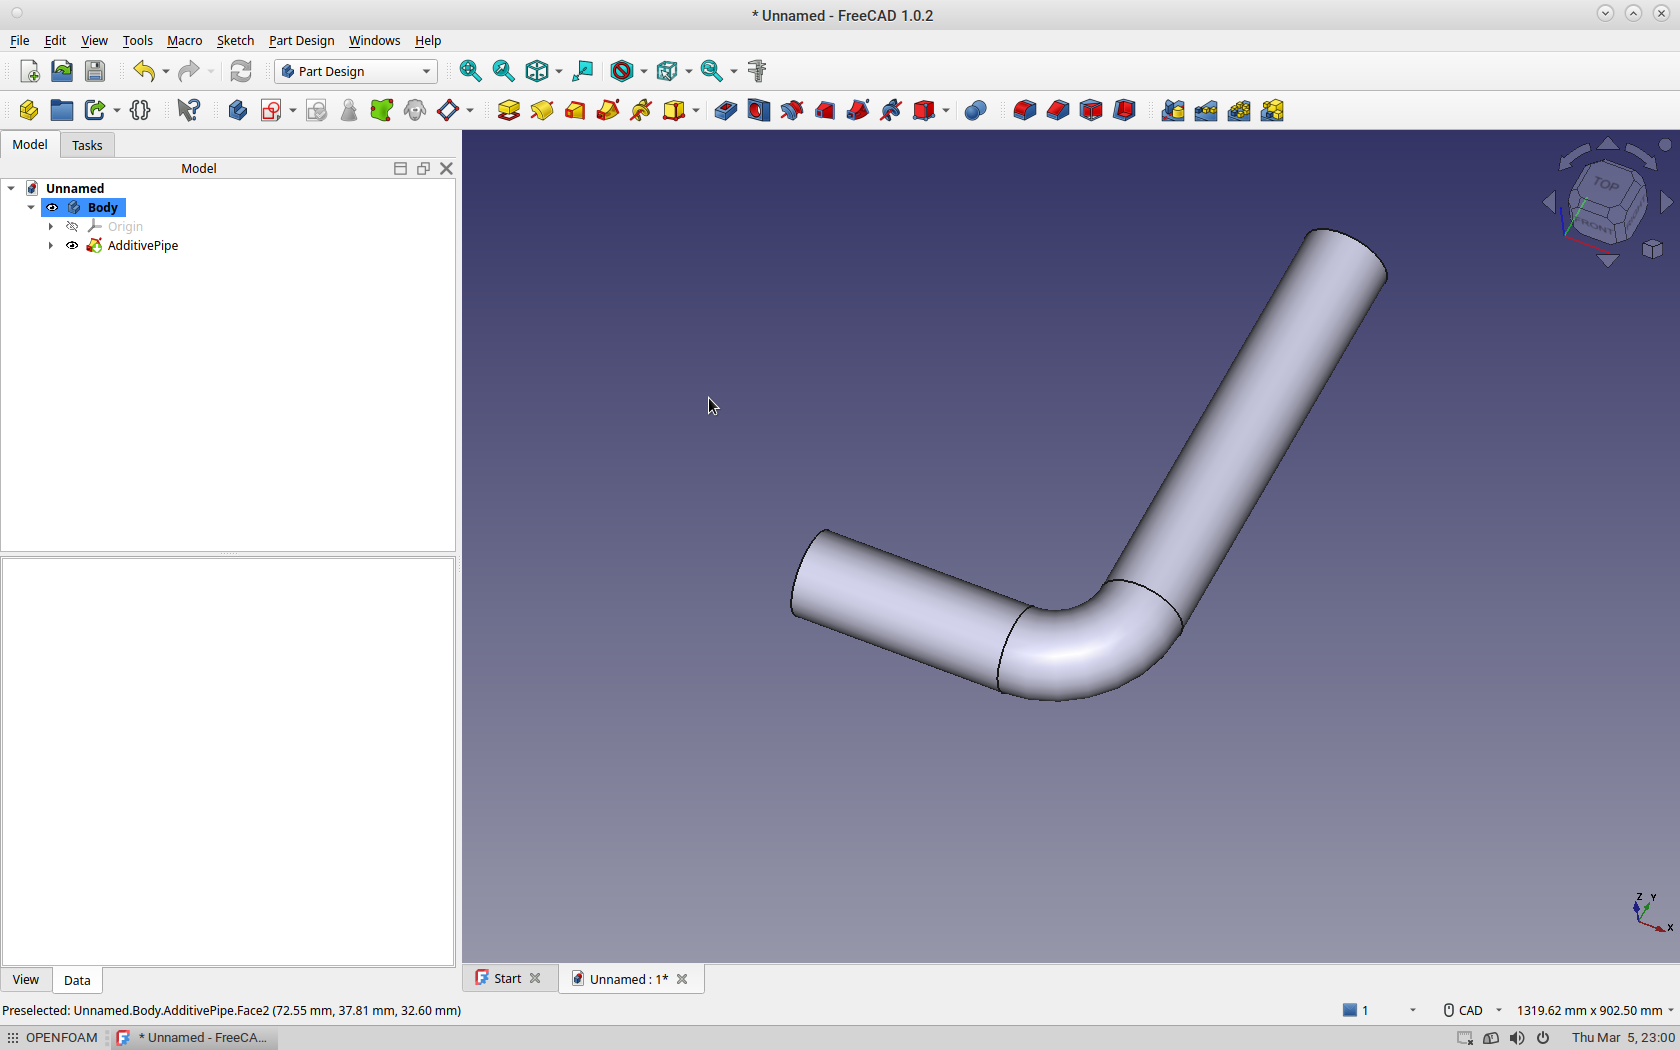
\includegraphics[width=0.7\linewidth]{pipe1}
		\caption{First main pipe}
		\label{fig:pipe1}
	\end{figure}
	
	Let's now make the secondary branch. Create another sketch, but in the \texttt{outlet}
	face, with a \qty{50}{mm} diameter circle, with center
	 coincident to $x$ axis, and  \qty{350}{mm} away from $z$ axis (see Figure 
	 \ref{fig:sketch2})
	 
	 \begin{figure}[h]
	 	\centering
	 	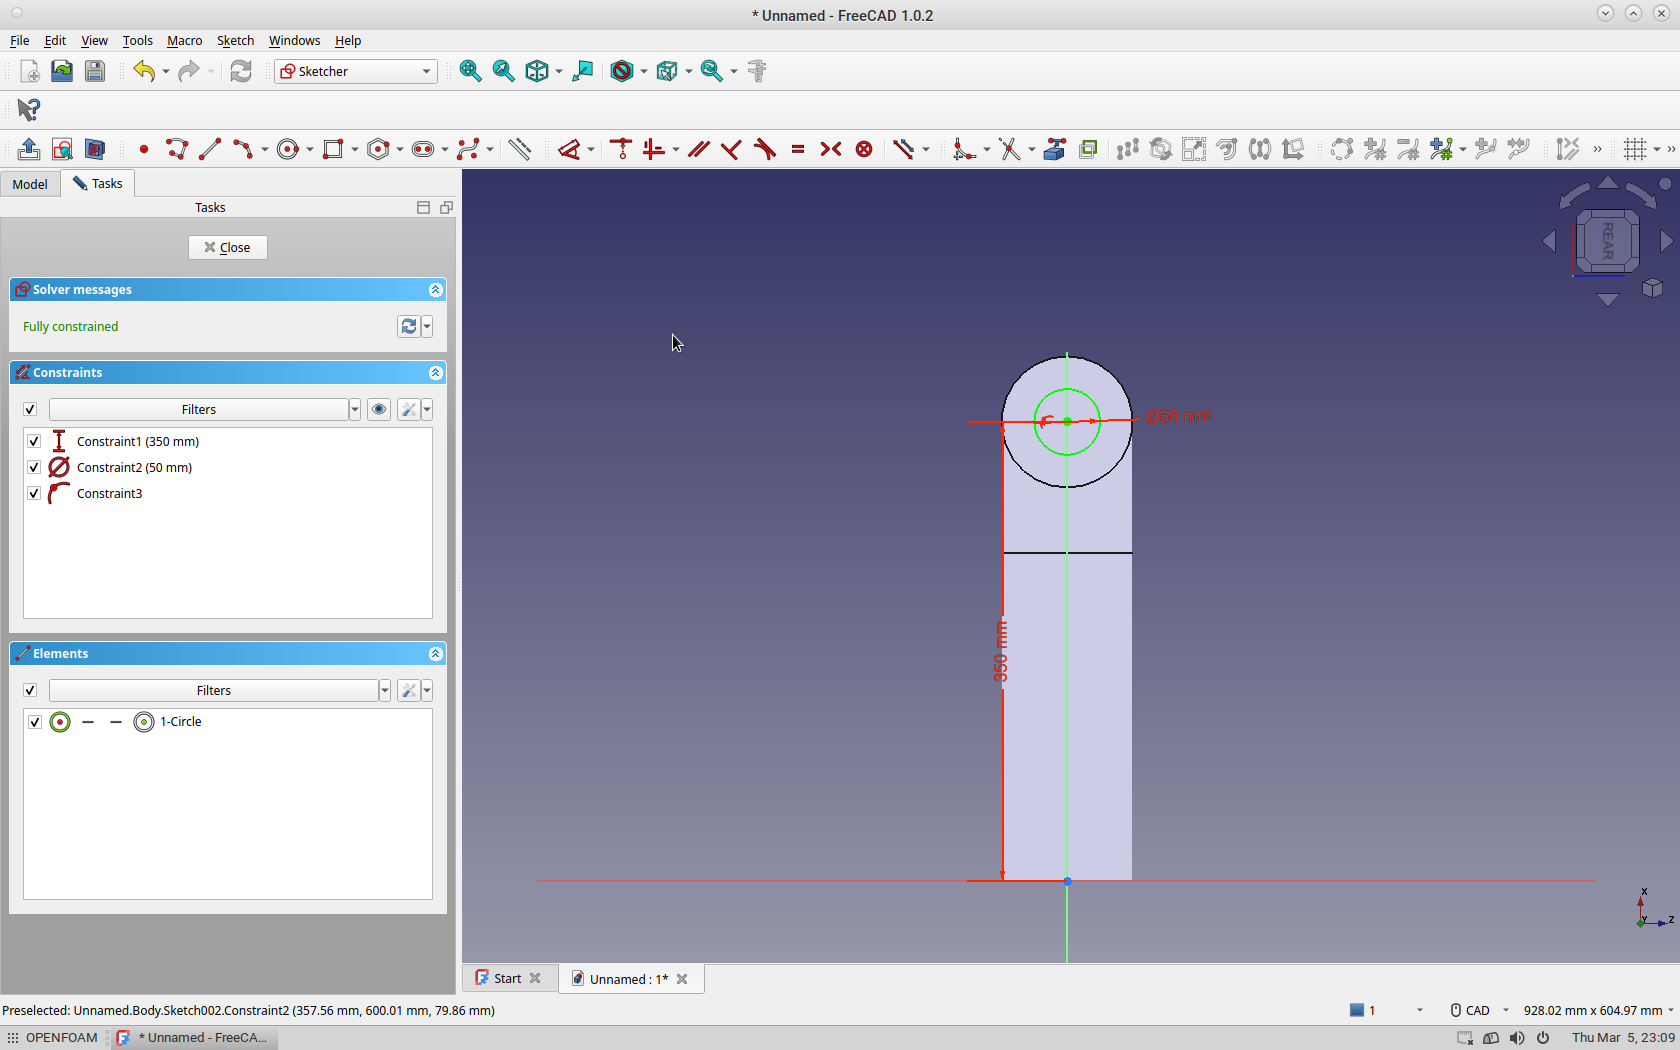
\includegraphics[width=0.7\linewidth]{sketch2}
	 	\caption{Circle in outlet face.}
	 	\label{fig:sketch2}
	 \end{figure}
	 
	 Make a \texttt{Pad} of \qty{800}{mm} with this circle with reversed direction, and the geometry is finished. \textbf{Don't forget to save the work!}. Save it with the name \texttt{Ypipe} in a \filename{Tutorial4} folder.
	 
	 \begin{figure}[h]
	 	\centering
	 	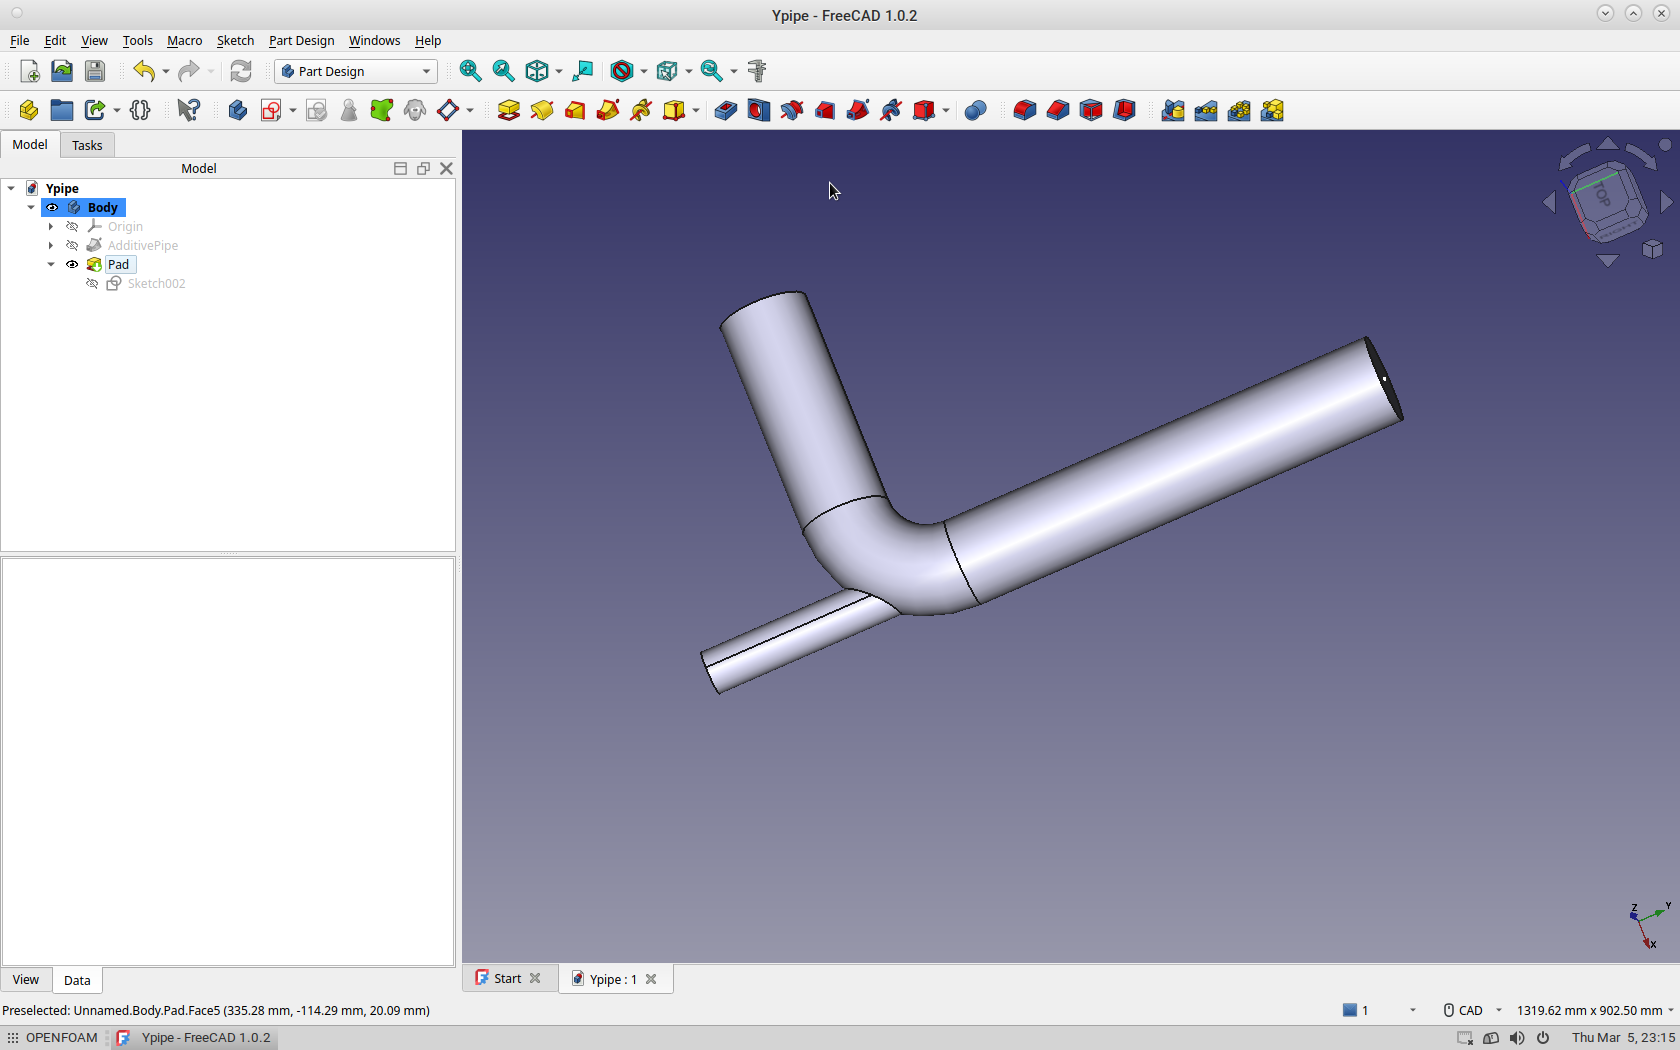
\includegraphics[width=0.7\linewidth]{pipe2}
	 	\caption{Y-pipe geometry.}
	 	\label{fig:pipe2}
	 \end{figure}
	 
	 \subsection{The shell}
	 
	 So far we have generated the solid, but OpenFOAM needs to read the mesh, that is, the 
	 surface around the solid, with a proper format. The most usual formats for this surface
	 are \href{https://en.wikipedia.org/wiki/STL_(file_format)}{Stereolithography (STL)} 
	 and \href{https://en.wikipedia.org/wiki/Wavefront_.obj_file}{Wavefront OBJ}. The 
	 latter is usually the most convenient, specially for large and complex geometries, 
	 because the smaller size of the file.
	 
	 First, explode the \texttt{Pad} part with the \texttt{Explode compound} tool in the 
	 \texttt{Part} workbench (see Figure \ref{fig:explode1}) 
	 
	 \begin{figure}[h]
	 	\centering
	 	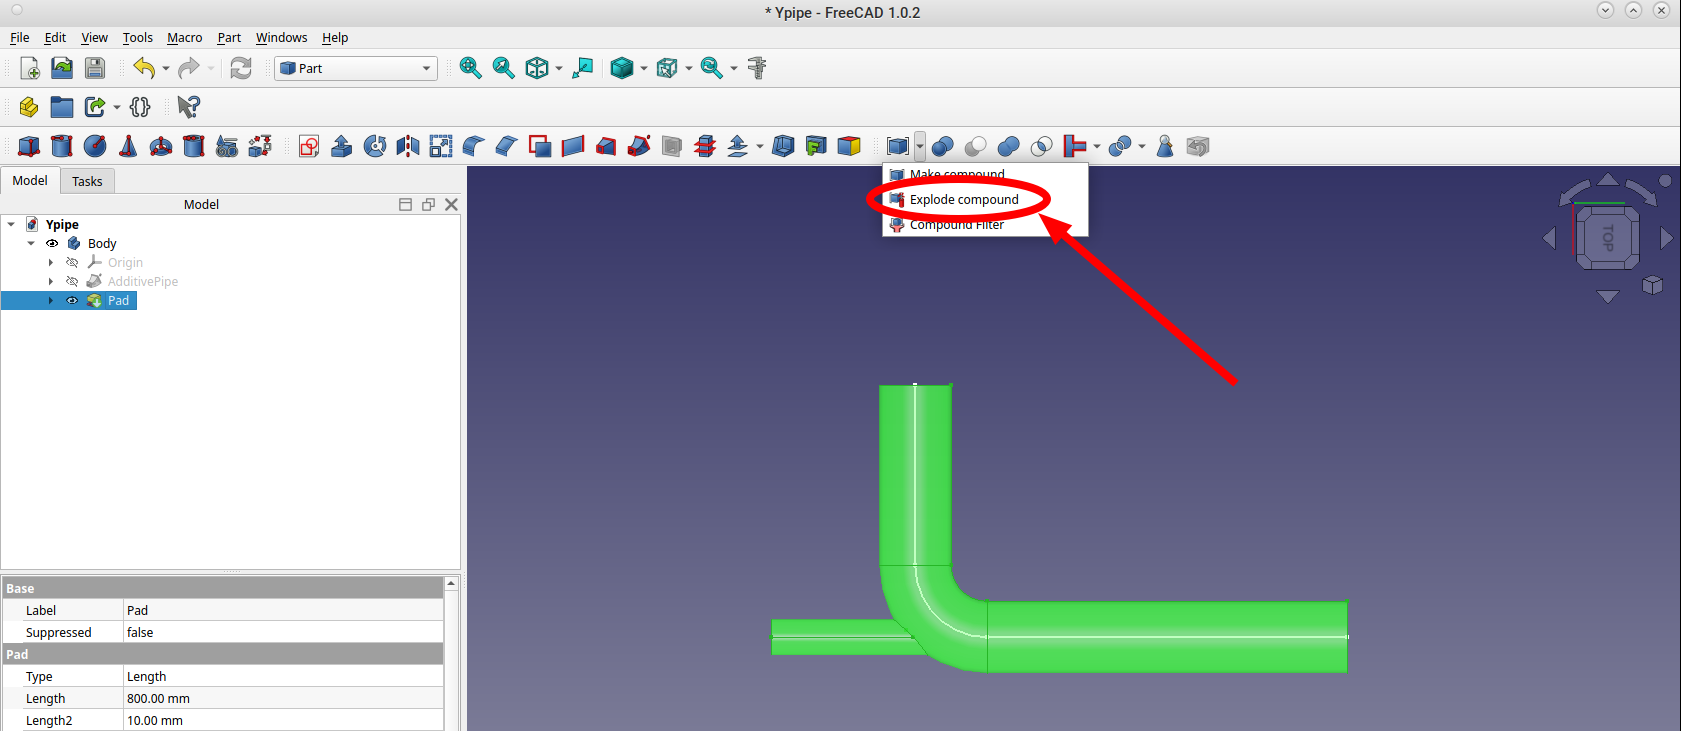
\includegraphics[width=0.7\linewidth]{explode1}
	 	\caption{First explode of \texttt{Pad} part.}
	 	\label{fig:explode1}
	 \end{figure}
	 
	 A \texttt{Pad.0} element, with the shell of the part, is created. The \texttt{Explode
	 compound} tool has to be applied on this element again in order to get the seven faces
	 of the solid.
	 
	 \begin{figure}[h]
	 	\centering
	 	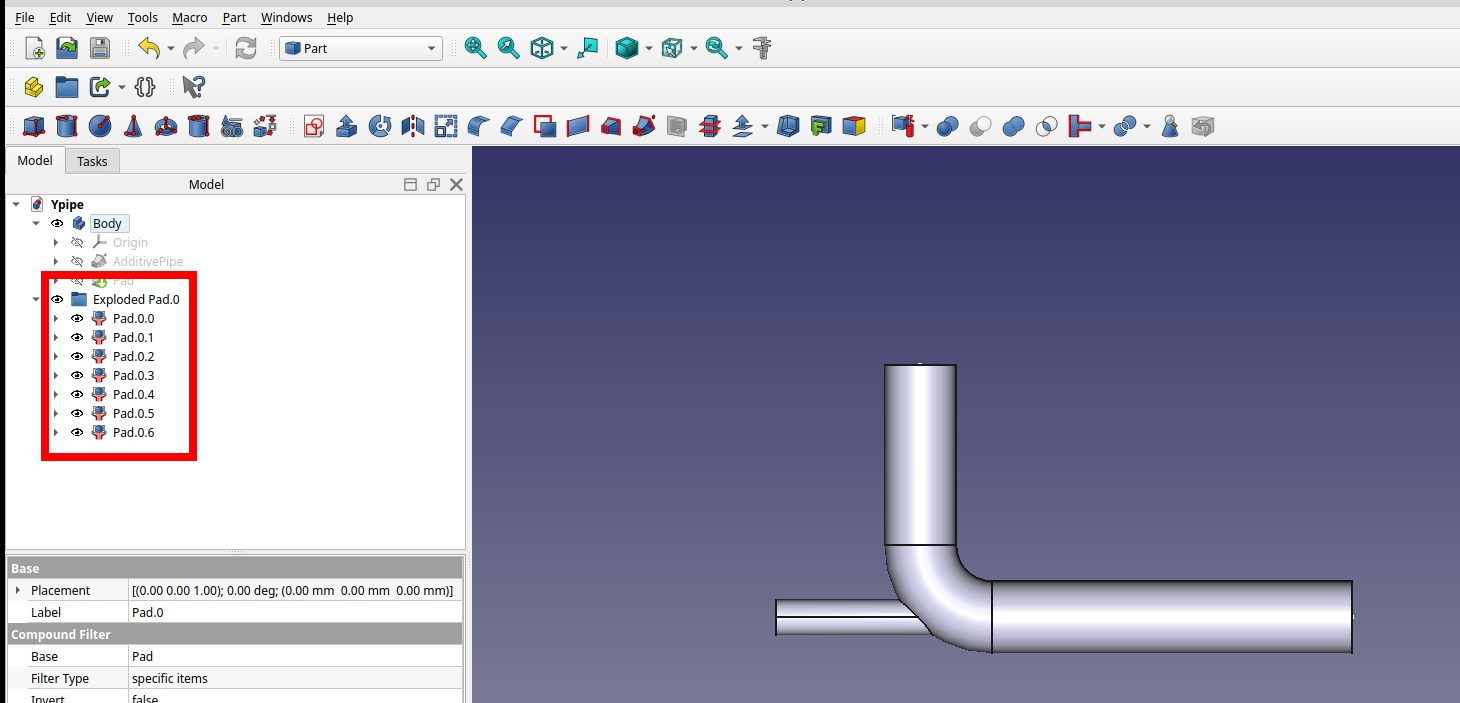
\includegraphics[width=0.7\linewidth]{explode2}
	 	\caption{Second explode of the \texttt{Pad} part.}
	 	\label{fig:explode2}
	 \end{figure}
	 
	 With \texttt{F2}, or \texttt{Rename} option in menu, the names of the faces can be 
	 modified:
	 \begin{itemize}
	 	\item \texttt{Pad.0} $\to$ \texttt{inlet1}
	 	\item \texttt{Pad.5} $\to$ \texttt{inlet2}
	 	\item \texttt{Pad.6} $\to$ \texttt{outlet}
	 \end{itemize}
	 
	 The four elements \texttt{Pad.0.X} that compose the wall shell have to be grouped in 
	 an only element with the \texttt{Make compound} command
	 
	 \begin{figure}[h]
	 	\centering
	 	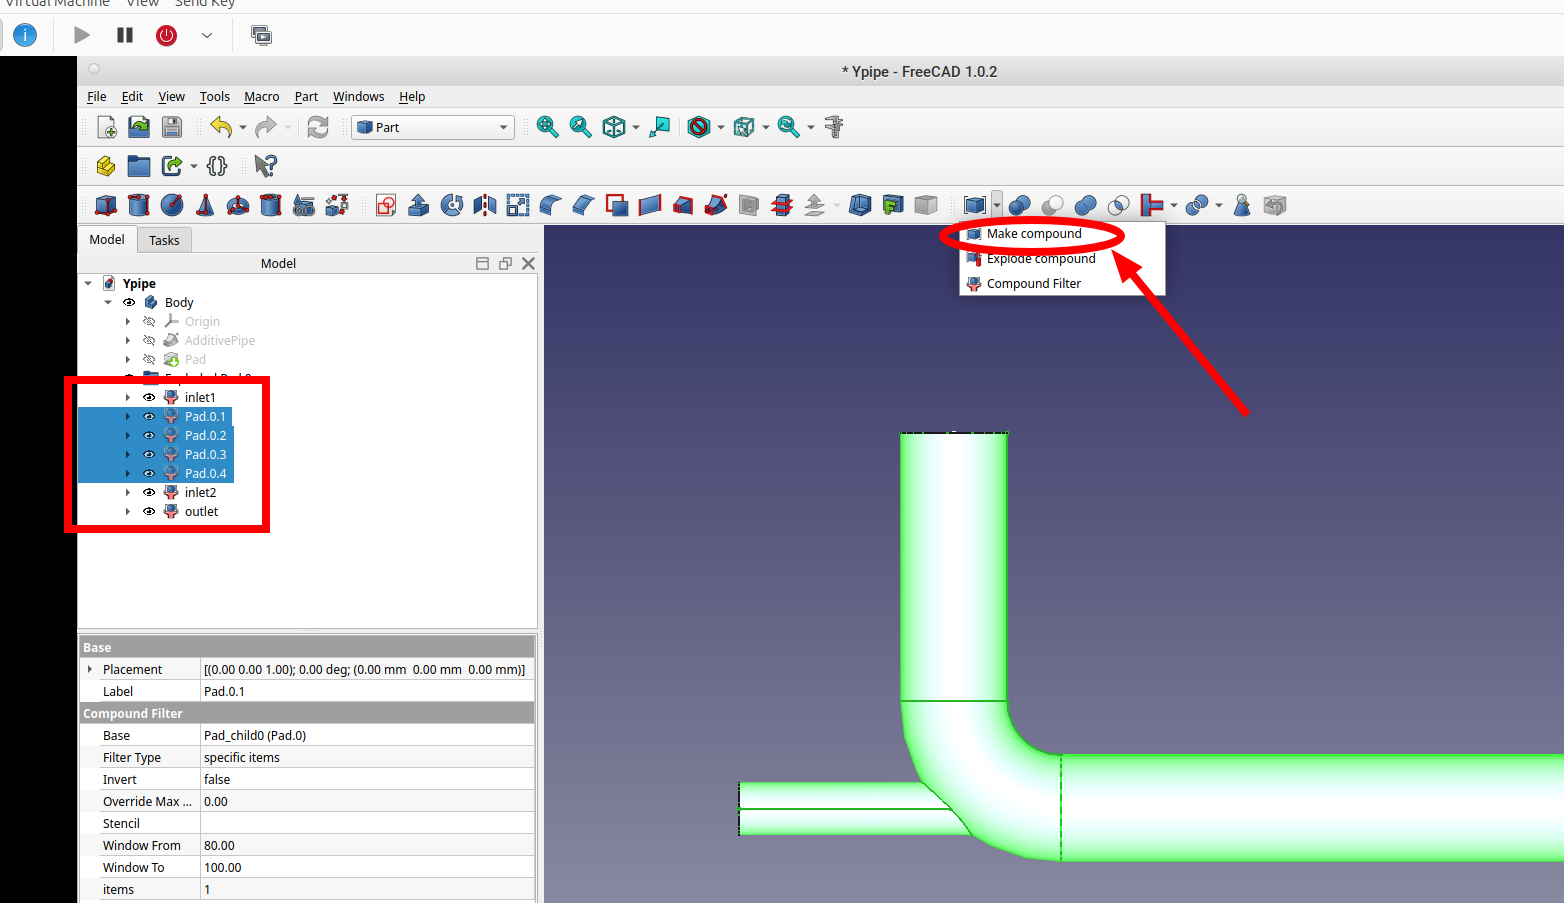
\includegraphics[width=0.7\linewidth]{compound}
	 	\caption{Making compound for the wall patch}
	 	\label{fig:compound}
	 \end{figure}
	 
	 Rename this new element
	 \begin{itemize}
	 	\item \texttt{Compound} $\to$ \texttt{wall}
	 \end{itemize}
	 
	 \subsection{The mesh}
	 Open the \texttt{Shell} workbench and create a mesh from the four shapes. Use \texttt{Mefisto} with \qty{10}{mm} of \texttt{Maximum edge length}
	 
	 \begin{figure}[h]
	 	\centering
	 	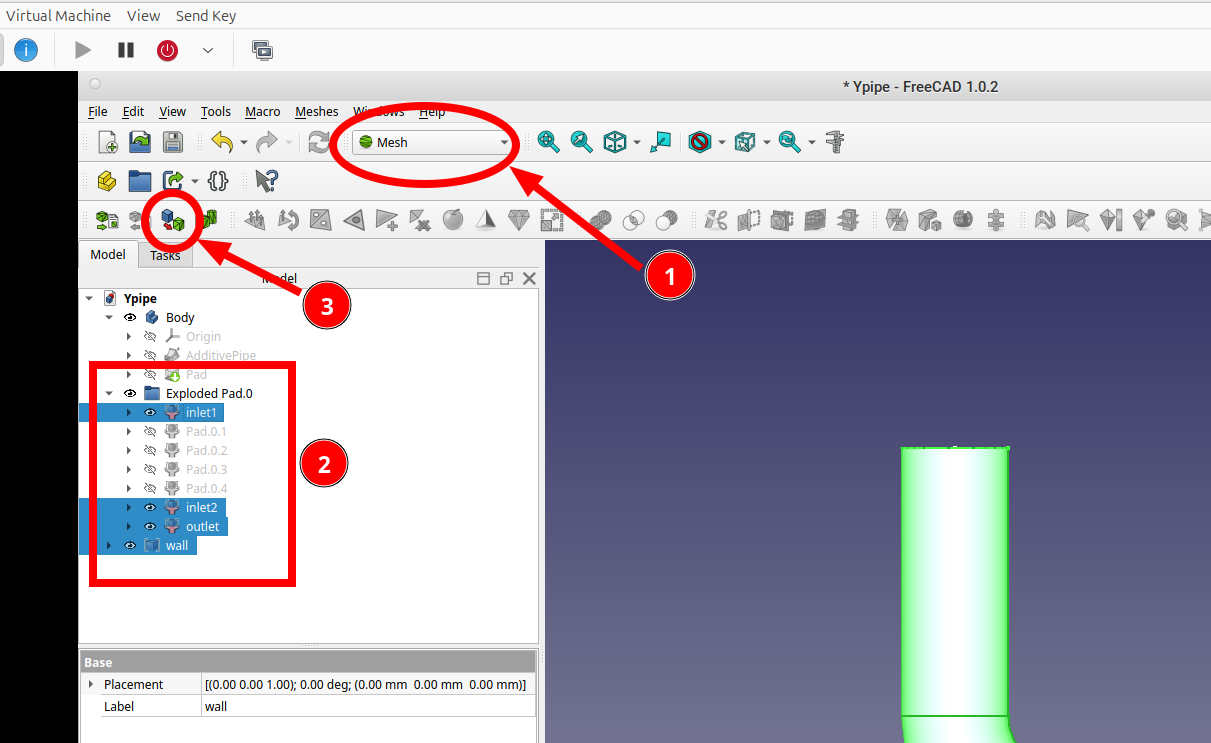
\includegraphics[width=0.7\linewidth]{mesh}
	 	\caption{Creating a mesh from the shapes.}
	 	\label{fig:mesh}
	 \end{figure}
	 
	 
	 	 This four meshes can now be exported as \texttt{ASCII STL}, removing the
	 	 \texttt{(Meshed)} part in the file name. It has to be done with the meshes one by
	 	 one (see Figure \ref{fig:meshexport}). Put the meshes in the folder
	 	 \filename{~/Tutorials/Tutorial\_4}, creating it if needed.
	 
	 \begin{figure}[h]
	 	\centering
	 	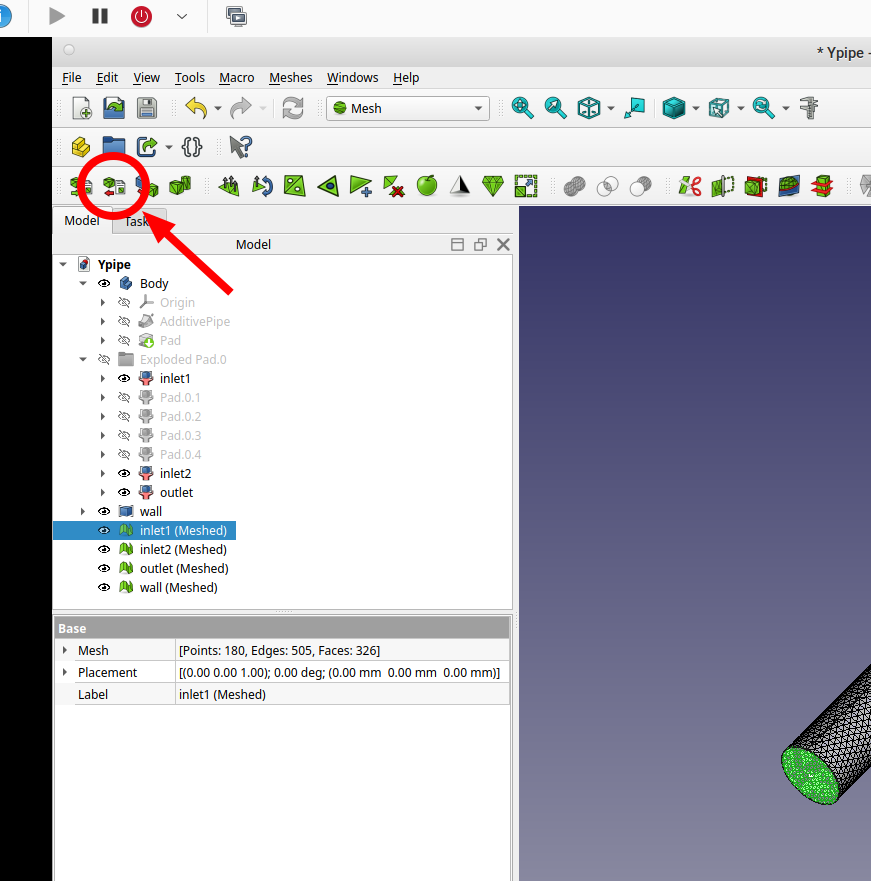
\includegraphics[width=0.5\linewidth]{mesh_export}
	 	\caption{Exporting the meshes}
	 	\label{fig:meshexport}
	 \end{figure}
	 
	 The part with \texttt{FreeCAD} is over. Now we continue with terminal commands. The
	 session in \texttt{FreeCAD} can be saved and the program can be closed.
	 
	\section{Setup of the case}
	
	Like in Tutorial \#3, simulation of orifice plate, we are going to use the \texttt{inflowOutflow} template case.
	
	\begin{lstlisting}[style=terminal]
		# load OpenFOAM if it is not included in the .bashrc file
		source /usr/lib/openfoam/openfoam-2312/etc/bashrc
		
		# Copy the inflowOutflow in this folder
		cp -r $FOAM_ETC/templates/inflowOutflow ~/Tutorials/Tutorial_3/Ypipe
		# Note that we have changed the name with the copy
		
		# Go to the tutorial place
		cd ~/Tutorials/Tutorial_3/Ypipe
	\end{lstlisting}
	
	We are going to mesh the Ypipe geometry with \terminalcmd{snappyHexMesh}. Read the \filename{README} file in the case for details. 
	
	\terminalcmd{snappyHexMesh} is very powerful and the result is usually a high
	quality mesh. But it requires skills, time and patience in order to use it correctly.  
	
	The presentation \cite{Jackson2012} gives a very detailed description of the program,
	 although a little outdated. Web page \cite{Thawtar2024} is also 
	a useful document with hints for using \terminalcmd{snappyHexMesh} 
	
	Basically, in order to make the mesh \terminalcmd{snappyHexMesh} needs three elements in the 
	case:
	\begin{itemize}
		\item A surface file, in format STL or OBJ, placed in the folder
		\filename{constant/triSurface}.
		\item A background structured mesh, usually provided by \terminalcmd{blockMesh}.
		\item A dictionary \filename{snappyHexMesDict}, placed in \filename{system} directory, 
		with all the parameter needed by \terminalcmd{snappyHexMesh} to make the mesh.
	\end{itemize}
	
	\subsection{Preparation of the surface file}
	
	Move the four \filename{*.stl} files generated with FreeCAD to the \filename{constant/triSurface} folder and perform the operations listed 
	in Listing \ref{lst:surface}.
	
	\begin{lstlisting}[style=terminal, caption={Preparation of the surface file.}, 
		label={lst:surface}]
		# We are considering that the STL files are in the Tutorial_4 folder
		mv ../*.stl constant/triSurface
		
		# Go to the folder to continue the work there and remove the template file
		cd constant/triSurface
		rm CAD.obj
		
		# Convert STL files to OBJ format. The option -clean, obviously cleans the 
		# surface file in the process
		surfaceConvert -clean inlet1.stl inlet1.obj
		surfaceConvert -clean inlet2.stl inlet2.obj
		surfaceConvert -clean outlet.stl outlet.obj
		surfaceConvert -clean wall.stl wall.obj
		
		# The STL files can now be removed, if desired
		rm *.stl
		
		# The four surfaces are joined in only one surface with four regions
		surfaceAdd inlet1.obj inlet2.obj Ypipe.obj
		surfaceAdd Ypipe.obj outlet.obj Ypipe.obj
		surfaceAdd Ypipe.obj wall.obj Ypipe.obj
		
		# The individual OBJ files can now be removed as well
		rm inlet*.obj outlet.obj wall.obj
		
	\end{lstlisting}
	
	\warning{The surface has been created in \texttt{FreeCAD} in \textbf{millimeters}, but 
	OpenFOAM works by default in International System, that is, with \textbf{meters}. We have to scale the surface}
	
	\begin{lstlisting}[style=terminal, caption={Scale of the surface file.}]
		# surfaceTransfromPoint -scale <scale factor> <input file> <output file>
		# scale factor can be a vector or an scalar
		# input and output files can be the same
		surfaceTransformPoints -scale 0.001 Ypipe.obj Ypipe.obj
	\end{lstlisting}
	
	Note that the regions in \filename{Ypipe.obj} fiel have still an annoying \texttt{(Meshed)} 
	in the name. We can easily get rid of this with the stream editor \terminalcmd{sed}.
	
	\begin{lstlisting}[style=terminal, caption={Removing the \texttt{(Meshed)} in the surface file.}]
		# just for checking, print the lines where ther is a (Meshed) region
		grep '(Meshed)' Ypipe.obj
		
		# Remove the expression
		sed -i 's/(Meshed)//g' Ypipe.obj
	\end{lstlisting}
	
	\tip{\terminalcmd{sed} is a simple but powerful program to process text files. In this command, \texttt{-i} option is for 'interactive', the output file is the same as the input file, and the expression \texttt{'s/<A>/<B>/g'} substitutes \texttt{<A>} by \texttt{<B>} in all 
	the occurrences in the file (\texttt{s} is for \texttt{\textbf{s}ubstitute} and \texttt{g} for \texttt{\textbf{`}lobal}, the entire file, not only the first occurrence).}
	
	The last step is just to check the surface file and get the bounding box to use with \terminalcmd{blockMesh}.
	
	\begin{lstlisting}[style=terminal]
		# check and print the bounding box
		surfaceCheck -blockMesh Ypipe.obj
	\end{lstlisting}
	
	Note the output of this command:
	
	\begin{lstlisting}[style=output]
		...
		
		vertices
		(
		(0 -0.2 -0.05)
		(0.4 -0.2 -0.05)
		(0.4 0.6 -0.05)
		(0 0.6 -0.05)
		(0 -0.2 0.05)
		(0.4 -0.2 0.05)
		(0.4 0.6 0.05)
		(0 0.6 0.05)
		);
		...
		
	\end{lstlisting}
	
	\subsection{The background mesh}
	
	With the output of the last command we modify the \filename{system/blockMeshDict} as in listing \ref{lst:blockMeshDict}
	
	
	\begin{lstlisting}[style=output, caption={\texttt{blockMeshDict} section of variables definition}, label={lst:blockMeshDict}]
	...
	backgroundMesh
	{
		xMin    0;
		xMax     0.4;
		yMin    -0.2;
		yMax     0.6;
		zMin    -0.05;
		zMax     0.05;
		xCells  20;
		yCells  40;
		zCells  5;
	}
	...	
	\end{lstlisting}
	
	Create the block mesh and visualize it along with the surface file to check that 
	everything is right.
	
	\begin{lstlisting}[style=terminal]
		foamJob -s -log-app blockMesh
		paraFoam
	\end{lstlisting}
	
	It should look like in Figure \ref{fig:blockMesh}.
	
	\begin{figure}[h]
		\centering
		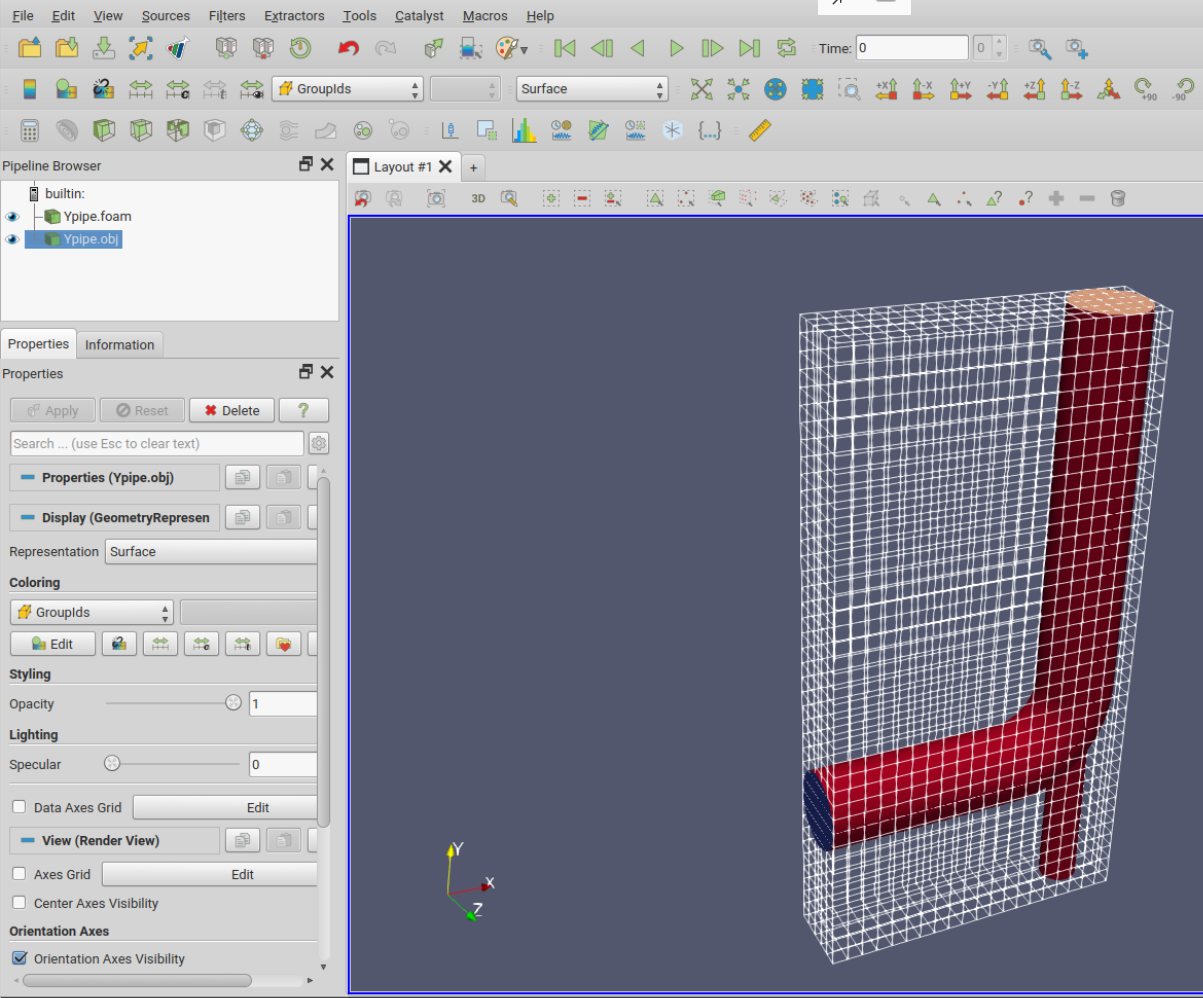
\includegraphics[width=\linewidth]{parafoam}
		\caption{Block mesh and the surface for the geometry}
		\label{fig:blockMesh}
	\end{figure}
	
	
	\subsection{Generation of the mesh}
	
	The program \terminalcmd{snappyHexMesh} makes the mesh in three stages:
	\begin{enumerate}
		\item \texttt{castellated} It refines the background mesh and defines the patches 
		according to the parameter
		provided by the dictionary. The result is something reminiscent of Minecraft.
		\item \texttt{snappy} It deforms the castellated mesh to fit the surface geometry.
		\item \texttt{addLayer} Insert cell layers to resolve boundary layer in the cells
		close to the walls.
	\end{enumerate}
	
	These stages can be enabled and disabled in the first section of the dictionary
	
	\begin{lstlisting}[style=output]
		...
		castellatedMesh on;
		snap            off;
		addLayers       off;
		...
	\end{lstlisting}
	
	\subsubsection{The castellated mesh}
	
	First, replace all the occurrences of \texttt{CAD} with \texttt{Ypipe} in the dictionary
	
	\begin{lstlisting}[style=terminal]
		sed -i 's/CAD/Ypipe/g' system/snappyHexMeshDict
	\end{lstlisting}
	
	Modify the \texttt{geometry} and \texttt{refinementSurfaces} subdictionaries as shown in Listing \ref{lst:geometry}.
	the \text
	
	\begin{lstlisting}[style=output, caption={\texttt{geometry} subdictionary},
		label={lst:geometry}]
	...
	geometry
	{
		Ypipe.obj
		{
			type triSurfaceMesh;
			name Ypipe;
			regions
			{
				inlet1  { name inlet1; }
				inlet2  { name inlet2; }
				outlet  { name outlet; }
				wall    { name wall;}
			}
		}
	};
	
	...

	refinementSurfaces
	{
		Ypipe
		{
			level (2 2);
			patchInfo { type wall; }
			
			regions
			{
				"inlet.*"
				{
					level (2 2);
					patchInfo
					{
						type patch;
						inGroups (inlet);
					}
				}
				
				outlet
				{
					level (2 2);
					patchInfo
					{
						type patch;
						inGroups (outlet);
					}
				}
			}
		}
	}
		\end{lstlisting}

\tip{For the refinement level definition, \texttt{(n m)} stands for \texttt{n} levels of 
refinement in the flat regions and \texttt{m} levels in corners.}

The rest of the \texttt{castellatedMesh} subdictionary can be keep as it is.

Run the mesher to perform this first stage.

	\begin{lstlisting}[style=terminal]
	foamJob -s -log-app snappyHexMesh
	
	# move the log to avoid the overwritting by other stages
	mv log.snappyHexMesh log.castellated
	\end{lstlisting}
	
	The result is written in folder \filename{1}, 
	and can be displayed with \terminalcmd{paraFoam} (see Figure \ref{fig:parafoam1}). 
	Probably you will understand now the reference to Minecraft.
	
	\begin{figure}[h]
		\centering
		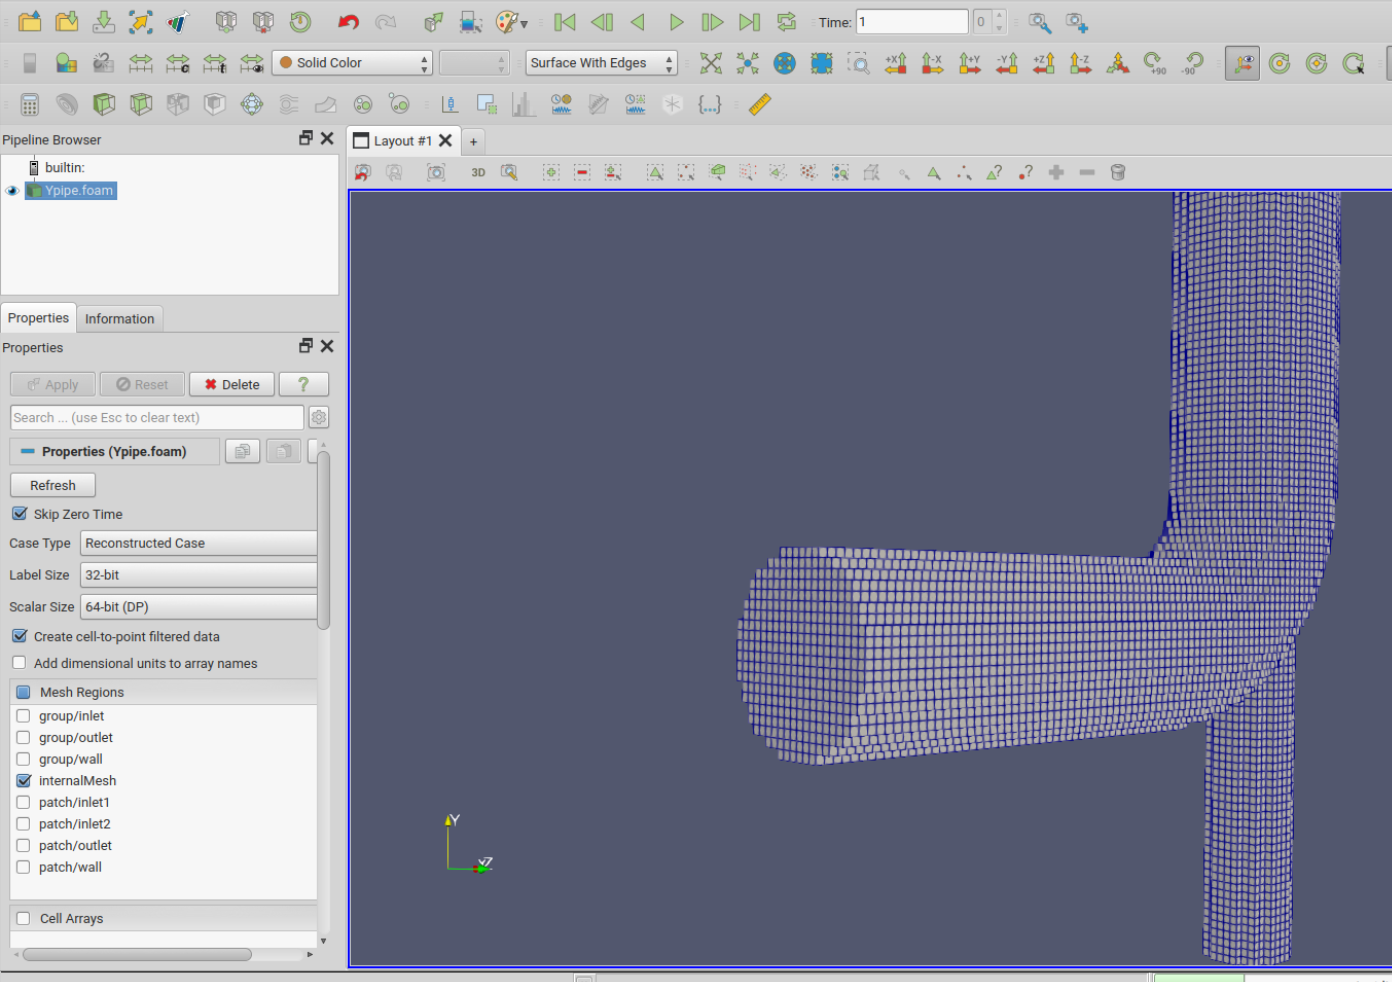
\includegraphics[width=1\linewidth]{parafoam1}
		\caption{Result of \texttt{castellated} stage.}
		\label{fig:parafoam1}
	\end{figure}
	
	\subsubsection{The snappy mesh}
	
	In order to perform the second stage, just enable it and disable the first one,
	
		\begin{lstlisting}[style=output]
		...
		castellatedMesh off;
		snap            on;
		addLayers       off;
		...
	\end{lstlisting}
	
	and run again the mesher
	
		\begin{lstlisting}[style=terminal]
		foamJob -s -log-app snappyHexMesh
		
		# move the log to avoid the overwritting by other stages
		mv log.snappyHexMesh log.snappy
	\end{lstlisting}
	
	Now the result is saved in the folder \filename{2}, and it looks like in the
	Figure \ref{fig:parafoam2}.
	
	\begin{figure}[h]
		\centering
		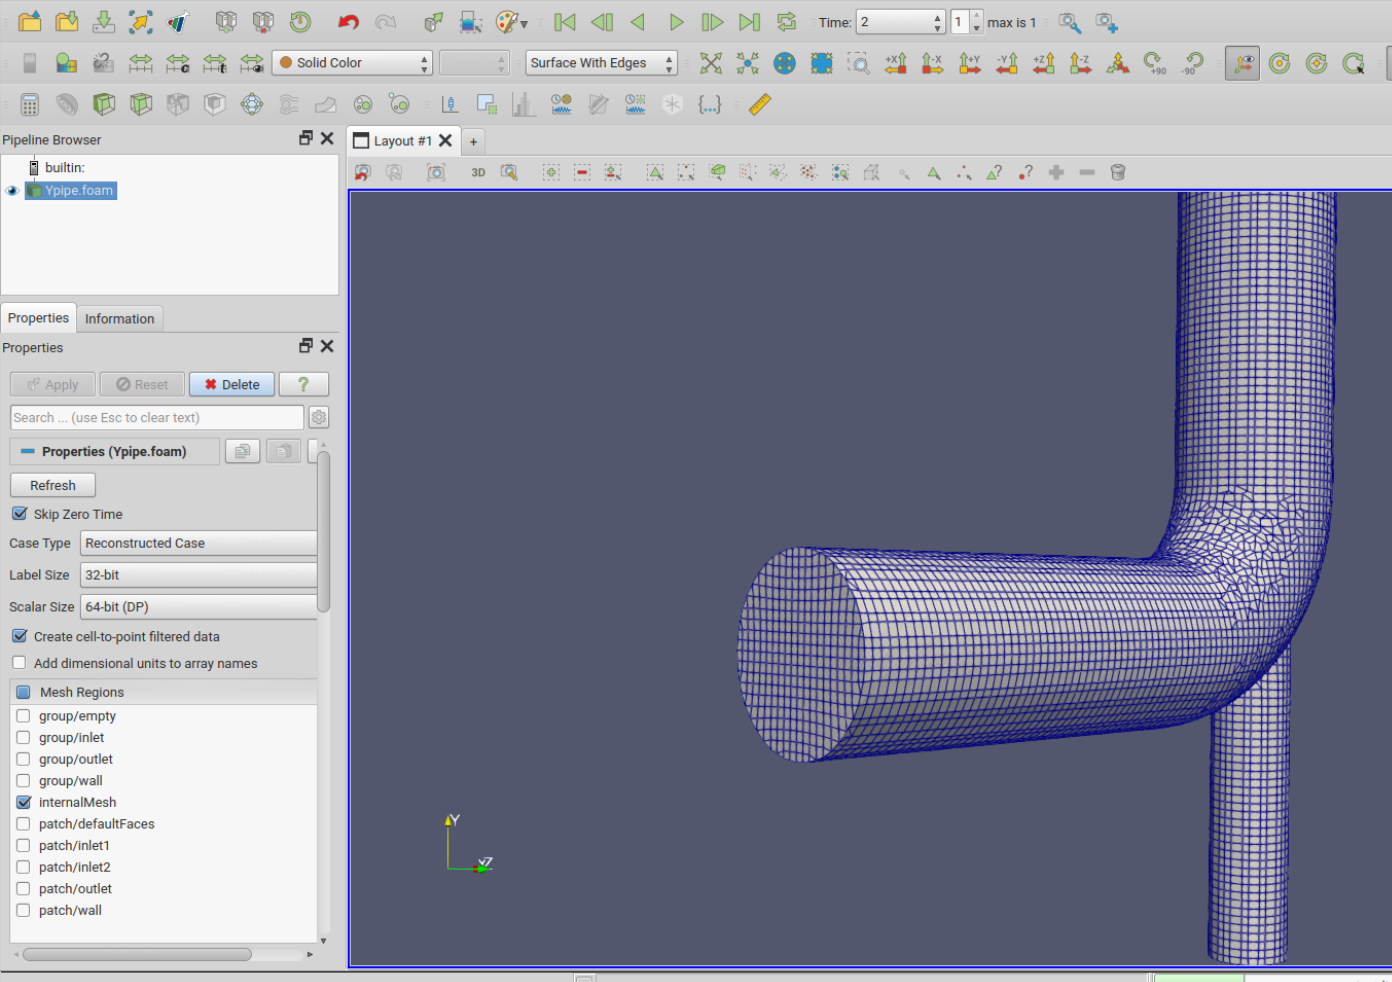
\includegraphics[width=1\linewidth]{parafoam2}
		\caption{Result of \texttt{snappy} stage.}
		\label{fig:parafoam2}
	\end{figure}
	
	\subsubsection{The mesh with layers}
	
	The last stage is done by enabling and modifying the \texttt{addLayerControls} 
	subdictionary
	
		\begin{lstlisting}[style=output]
		...
		castellatedMesh off;
		snap            off;
		addLayers       on;
		...
		addLayersControls
		{
			layers
			{
				"wall.*"
				{
					nSurfaceLayers 3;
				}
			}
			
			relativeSizes       true; // false, usually with firstLayerThickness
			expansionRatio      1.2;
			finalLayerThickness 0.5;
			minThickness        1e-3;
			//  firstLayerThickness 0.01;
			
			//  maxThicknessToMedialRatio 0.6;
		}
	\end{lstlisting}
	
	\begin{lstlisting}[style=terminal]
		foamJob -s -log-app snappyHexMesh
		
		# move the log to avoid the overwritting by other stages
		mv log.snappyHexMesh log.layers
	\end{lstlisting}
	
	The result is shown in Figure \ref{fig:parafoam3}.
	
	\begin{figure}[h]
		\centering
		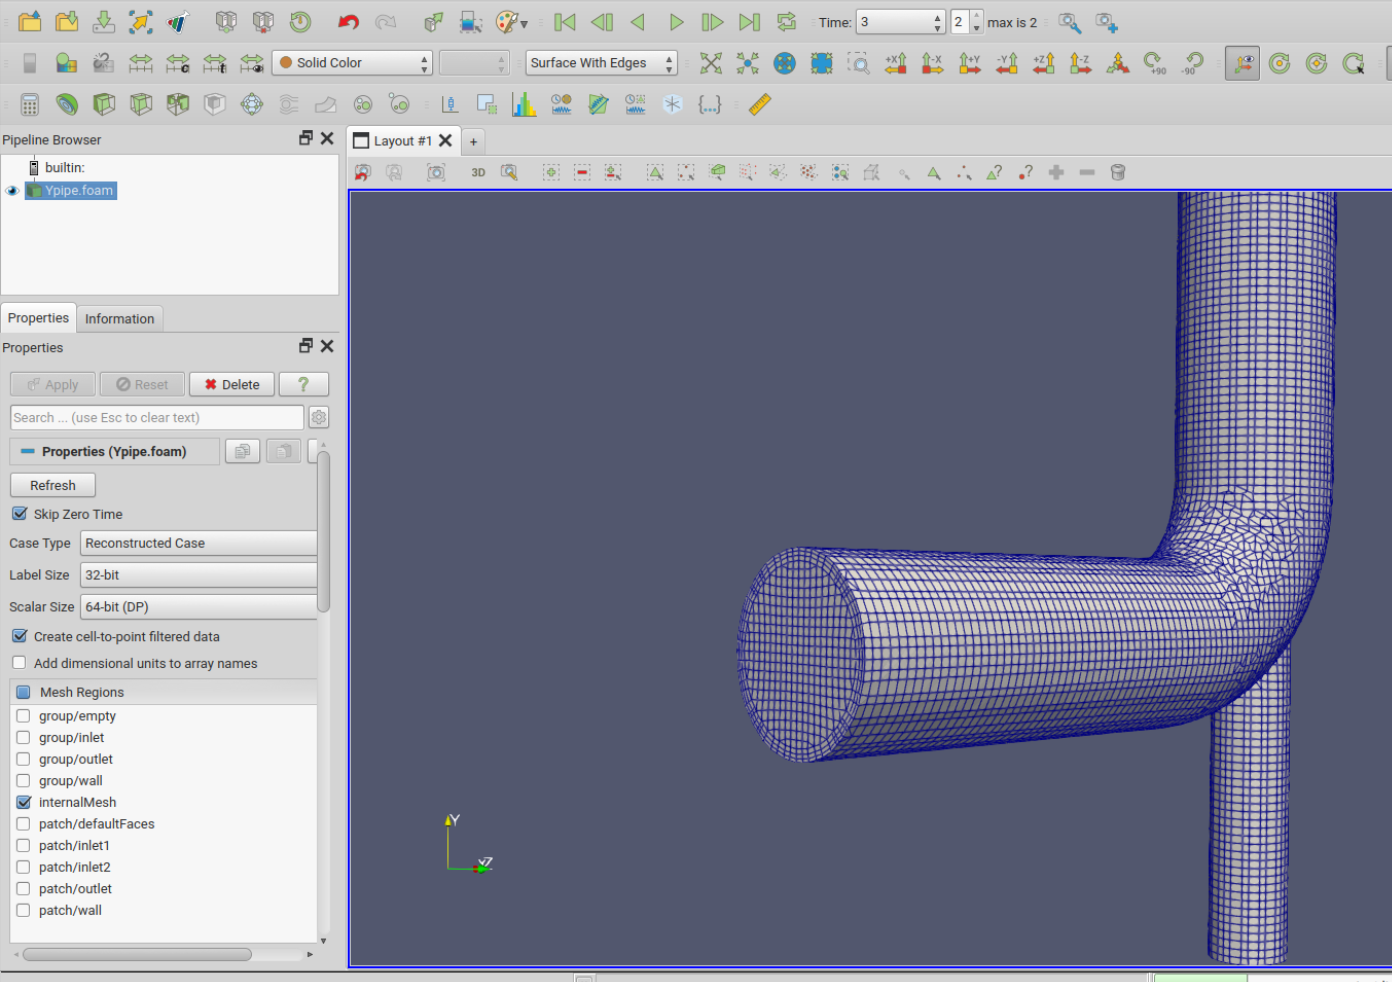
\includegraphics[width=\linewidth]{parafoam3}
		\caption{The mesh with layers in the wall.}
		\label{fig:parafoam3}
	\end{figure}
	
	 This mesh can now be placed in the \filename{constant} folder to be used with the simulation, and the intermediate stages can be removed
	 
	 \begin{lstlisting}[style=terminal]
	 	# Remove the block mesh
	 	rm -r constant/polyMesh
	 	
	 	# ... and replaced it by the definitive mesh
	 	mv 3/polyMesh constant
	 \end{lstlisting}
	 
	 \tip{\terminalcmd{snappyHexMesh} can be ran with the option \texttt{-overwrite} and all the stages \texttt{on}. Then it performs the three stages and overwrites the final
	 result on \filename{constant}. We have done this step by step for educational purposes and to shown how to control each stage.}
	 
	 \subsubsection{Mesh Quality Check}
	 
	 Before running the simulation, verify the mesh quality:
	 
	 \begin{lstlisting}[style=terminal]
	 	# Check mesh quality
	 	checkMesh
	 	
	 	# Look for these indicators:
	 	# - Max non-orthogonality < 70 (ideally < 65)
	 	# - Max skewness < 4
	 	# - Number of faces with high aspect ratio (optional)
	 \end{lstlisting}
	 
	 If the mesh has issues, you may need to adjust the \filename{snappyHexMeshDict} parameters.
	 
	 \subsection{Boundary conditions and physical parameters}
	 
	 We have to add another \texttt{inlet} in all the files of the folder \filename{0}.
	 
	 \begin{lstlisting}[style=output, caption={0/U}]
	 Uinlet          (0 4 0);
	 
	 dimensions      [0 1 -1 0 0 0 0];
	 
	 internalField   uniform (0 0 0);
	 
	 boundaryField
	 {
	 	inlet1
	 	{
	 		type            pressureInletOutletVelocity;
	 		value           uniform (0 0 0);
	 	}
	 	
	 	inlet2
	 	{
	 		type            fixedValue;
	 		value           uniform $Uinlet;
	 	}
	 	
	 	outlet
	 	{
	 		type            pressureInletOutletVelocity;
	 		value           uniform (0 0 0);
	 	}
	 	
	 	wall
	 	{
	 		type            noSlip;
	 	}
	 	
	 	#includeEtc "caseDicts/setConstraintTypes"
	 }
	 \end{lstlisting}
	 
	 \begin{lstlisting}[style=output, caption={0/p}]
	 dimensions      [0 2 -2 0 0 0 0];
	 
	 internalField   uniform 0;
	 
	 boundaryField
	 {
	 	inlet1
	 	{
	 		type            fixedValue;
	 		value           uniform 0;
	 	}
	 	
	 	inlet2
	 	{
	 		type            zeroGradient;
	 	}
	 	
	 	outlet
	 	{
	 		type            fixedValue;
	 		value           uniform 0;
	 	}
	 	
	 	wall
	 	{
	 		type            zeroGradient;
	 	}
	 	
	 	#includeEtc "caseDicts/setConstraintTypes"
	 }
	\end{lstlisting}
	
		 \begin{lstlisting}[style=output, caption={0/k}]
		kInlet          0.00375;
		
		dimensions      [0 2 -2 0 0 0 0];
		
		internalField   uniform $kInlet;
		
		boundaryField
		{
			inlet1
			{
				type            inletOutlet;
				inletValue      uniform $kInlet;
				value           uniform $kInlet;
			}
			
			inlet2
			{
				type            turbulentIntensityKineticEnergyInlet;
				intensity       0.05;
				value           uniform $kInlet;
			}
			
			outlet
			{
				type            inletOutlet;
				inletValue      uniform $kInlet;
				value           uniform $kInlet;
			}
			
			wall
			{
				type            kqRWallFunction;
				value           uniform $kInlet;
			}
			
			#includeEtc "caseDicts/setConstraintTypes"
		}
	\end{lstlisting}
	
	\begin{lstlisting}[style=output, caption={0/omega}]
		omegaInlet      80.0;
		
		dimensions      [0 0 -1 0 0 0 0];
		
		internalField   uniform $omegaInlet;
		
		boundaryField
		{
			inlet1
			{
				type            inletOutlet;
				inletValue      uniform $omegaInlet;
				value           uniform $omegaInlet;
			}
			
			inlet2
			{
				type            turbulentMixingLengthFrequencyInlet;
				mixingLength    0.0035;
				value           uniform $omegaInlet;
			}
			
			outlet
			{
				type            inletOutlet;
				inletValue      uniform $omegaInlet;
				value           uniform $omegaInlet;
			}
			
			wall
			{
				type            omegaWallFunction;
				value           uniform $omegaInlet;
			}
			
			#includeEtc "caseDicts/setConstraintTypes"
		}
	\end{lstlisting}
	
	The fluid is water, like in Tutorial \#3. Modify \filename{constant/transportProperties} according to that.
	
	\subsection{Setting up the solver}
	
	Like in Tutorial \#3, we include the \texttt{solverInfo} function with the variables 
	\texttt{k} and \texttt{omega} added to the dictionary, and the function called from 
	\filename{system/controlDict}. Also, we include the \texttt{flowRatePatch} function,
	defining the patch \texttt{inlet1} in order to monitor the flow rate dragged
	by the flow in \texttt{inlet2}.
	
	\subsection{Solving the flow and main results}
	
	Run the solver with
	
	 \begin{lstlisting}[style=terminal]
		foamjob -s -log-app simpleFoam
	\end{lstlisting}
	
	The residuals are not very low, specially for pressure and turbulence magnitudes.
	 This is an usual trend for 
	pressure-driven flows.
	
	\begin{figure}[h]
		\centering
		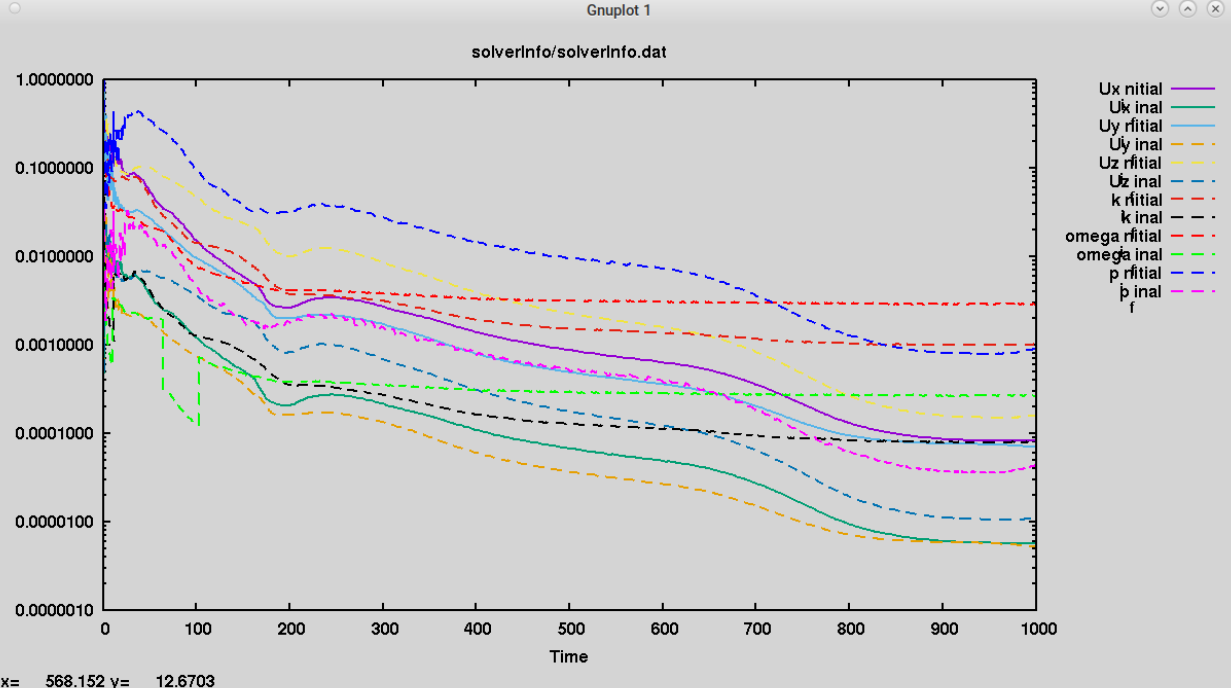
\includegraphics[width=0.7\linewidth]{residuals}
		\caption{Plot of residuals}
		\label{fig:residuals}
	\end{figure}
	
	The flow rate in \texttt{inlet1} converges quite quickly to its final
	value of, approximately, \qty{-0.008}{m^3/s}. The negative value means that it is an
	inlet flow.
	
	\subsection{Visualization in ParaView}
	
	Useful \texttt{ParaView} filters for this case:
	\begin{itemize}
		\item \textbf{Slice}: Create a plane through the pipe center to see internal flow
		\item \textbf{Stream Tracer}: Generate flow lines from the inlets
		\item \textbf{Clip}: Cut away half the pipe to see internal pressure distribution
		\item \textbf{Calculator}: Compute derived quantities like total pressure or vorticity
	\end{itemize}
	
	Contours of velocity and pressure are shown in Figure \ref{fig:pu}, and $k$ and $\omega$ in Figure \ref{fig:komega}.
	
	
	\begin{figure}[h]
		\centering
		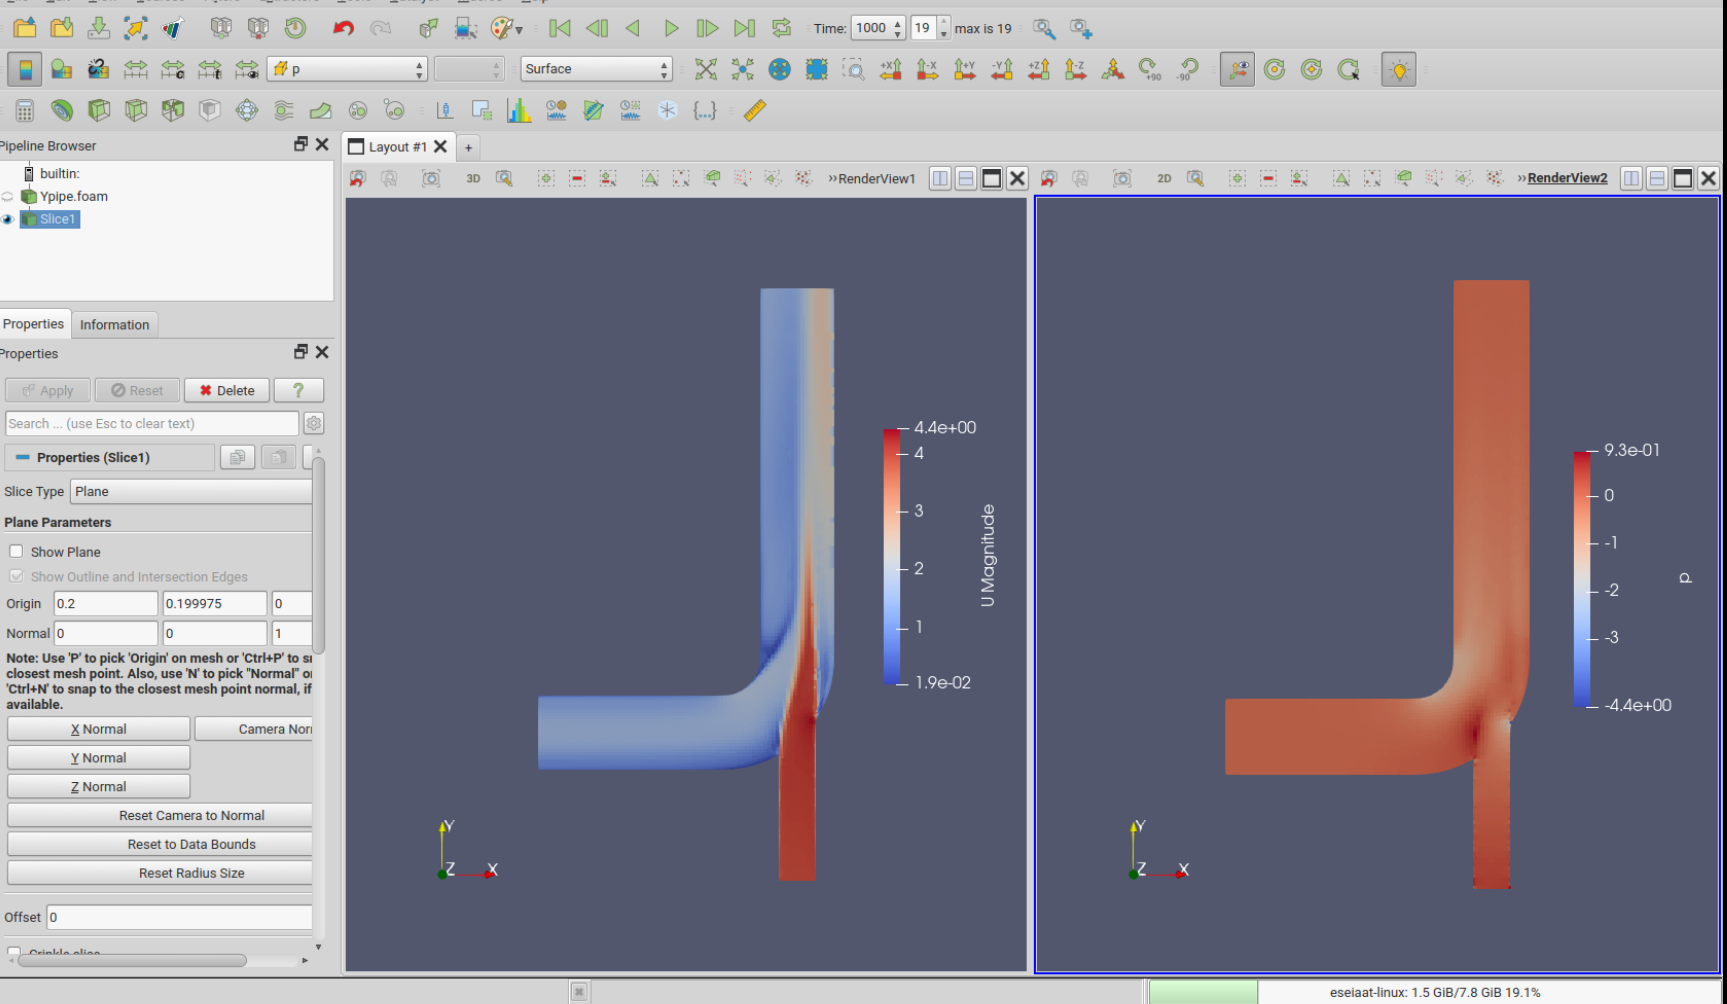
\includegraphics[width=\linewidth]{pU}
		\caption{Contours of velocity and pressure in the middle plane.}
		\label{fig:pu}
	\end{figure}
	
	\begin{figure}[h]
		\centering
		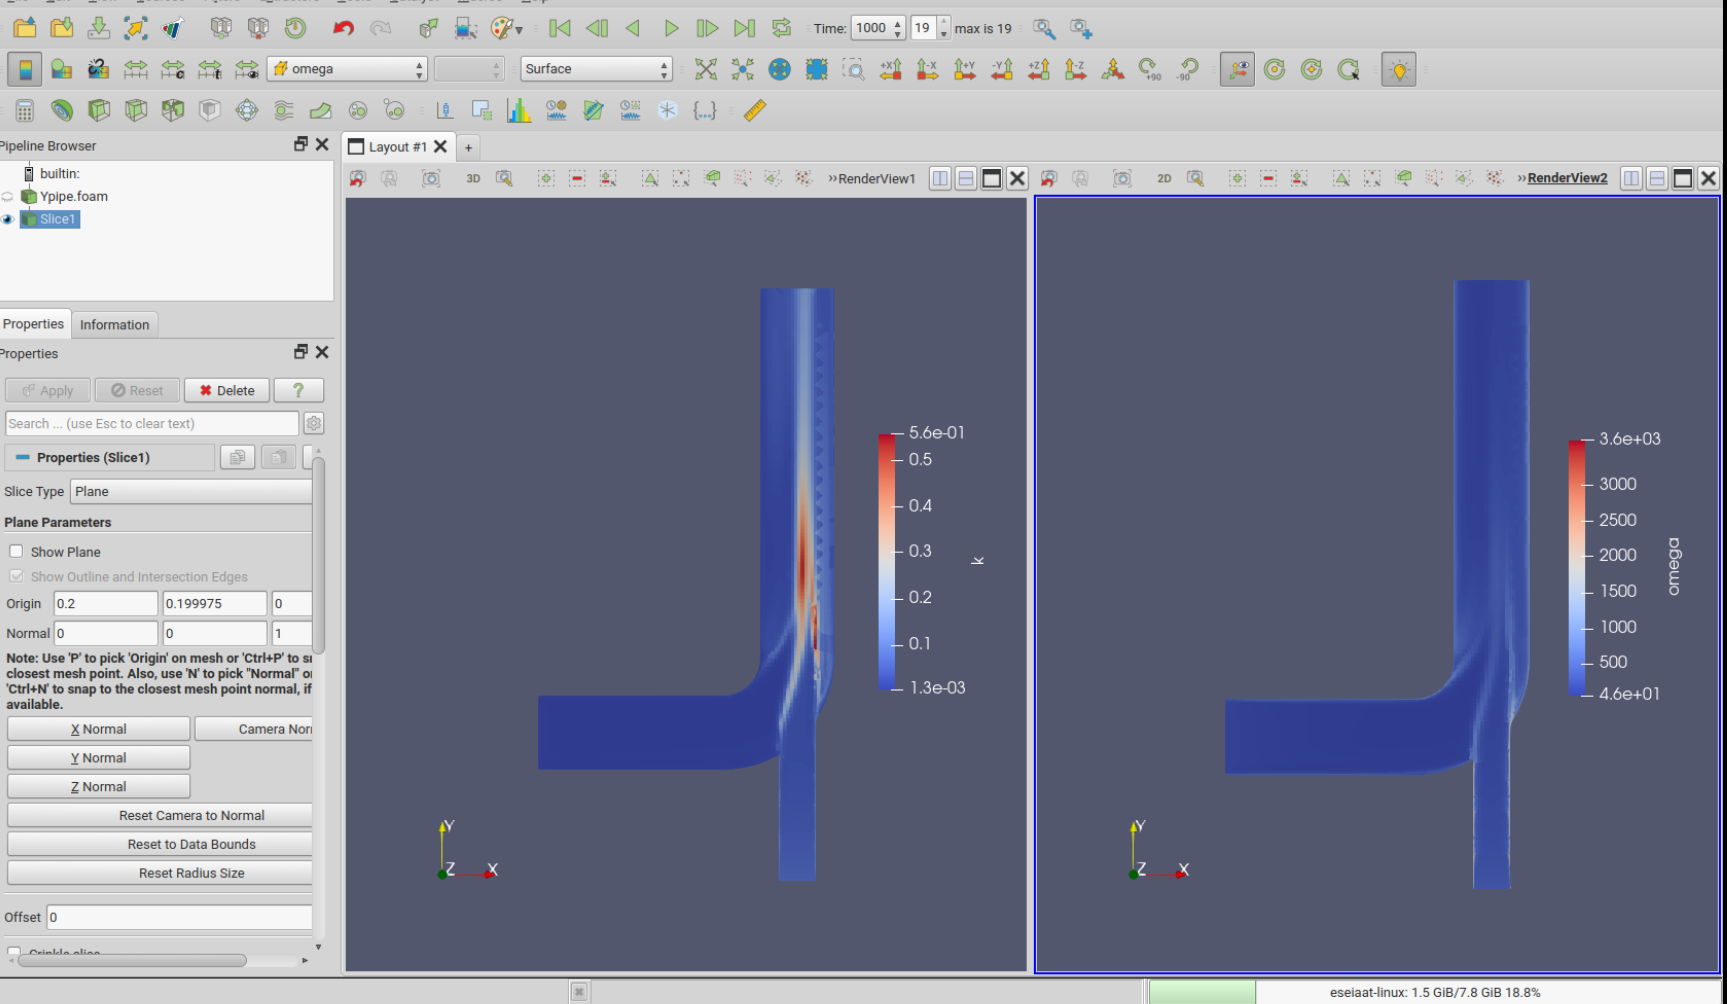
\includegraphics[width=\linewidth]{kOmega}
		\caption{Contours of $k$ and $\omega$ in the middle plane.}
		\label{fig:komega}
	\end{figure}
	
	\section{Exercises}
	
	\subsection{Modify pressure boundary conditions}
	
	The simulation has been conducted with fixed static boundary conditions in both \texttt{inlet1}
	and \texttt{outlet}. Nevertheless, it would be more correct to define both boundaries
	as \texttt{totalPressure}. Read the documentation for this boundary condition and 
	run again the simulation with both total pressures with value \qty{0}{m^2/s^2}
	
	\subsection{Modification of outlet pressure}
	
	The outlet pressure has ben defined like the inlet pressure, \qty{0}{m^2/s^2}. But
	this device acts like a pump, where the flow in \texttt{inlet1} is dragged against a
	adverse pressure gradient. Compute the flow rate when the \texttt{outlet} total pressure
	is larger than the inlet total pressure. 
	
	Consider that the outlet pressure is 
	$N\times \qty{0.1}{m^2/s^2}$, where $N$ is the number of your group.	
	
	\begin{thebibliography}{9}
		
	\bibitem{Jackson2012}
	Jackson A. (2012) \textit{A Comprehensive Tour of snappyHexMesh} 7th OpenFOAM Workshop
	\href{https://openfoamwiki.net/images/f/f0/Final-AndrewJacksonSlidesOFW7.pdf}{link} (Visited on March 2026)
	
	\bibitem{Thawtar2024}
	Thawtar (2024)	
	\href{https://cfdmonkey.com/tips-and-tricks-for-significantly-improving-your-snappyhexmesh/}
	{link}
	(Visited on March 2026)
	
	\end{thebibliography}
\end{document}